\subsection{进程调度}
导言:
计算机在运行的过程中,经常会出现这样一种情况,那就是内存中的可执行程序(进程)个数大于处理器的个数,为了使得这些程序都能完成自己的任务,处理器可以共享给这些程序使用。而操作系统在这其中起到的作用就是让这些进程高效合理的利用处理器资源,而这个过程我们称之为进程调度(scheduling)。进程调度是进程管理的重要组成部分。

我们的生活中处处存在调度,比如说食堂打饭,一个窗口的阿姨如何满足众多的食客,又比如一家工厂里的一台机床如何处理众多等待加工的零件。调度就是在一定的约束条件下,将有限的资源合理的分配给若干个任务,使得这些任务满足一些指标。回到我们要将的进程调度上,也就是在有限的cpu资源下,操作系统通过某种调度策略,使得各进程在时间上能够得到处理机完成自己的任务,并且满足一定的性能指标。

然而,NPUcore是如何完成这个看似简单的操作呢?接下来我们将阐述npucore的进程调度这个核心的问题。
\\[10pt]
5.2.4.1 调度策略

我们先大体介绍一下几种常用的调度策略,并详细说明npucore采用的调度策略。

(1)先来先服务:
先来先服务(first-come first-severed,FIFO,先进先出)调度策略的基本思想是按照进程请求处理器的先后顺序使用处理器。操作系统会创建两个队列,一个称之为就绪队列,一个称之为阻塞队列。

(2)最短作业优先(SJF):
在作业调度中,该算法每次从后备作业队列中挑选估计服务时间最短的一个或几个作业,将他们调入内存,分配必要的资源,创建进程并放入就绪队列。

(3)基于时间片的轮转:
如果操作系统给每个运行的进程的运行时间是一个足够小的时间片(time slice),时间片一到,就抢占当前进程并切换到另外一个进程进行执行。这样进程以时间片为单位轮流占用处理器执行。对于交互式进程而言,就有比较大的机会在较短时间内执行,从而有助于减少响应时间。这种调度策略称为时间片轮转(Round-Robin,RR)调度,基本思路即从就绪队列头取出一个进程,让他运行一个时间片,然后把它放回队列尾,再从队列头取下一个进程执行,周而复始。

(4)多级反馈队列调度:
操作系统根据进程过去一段的执行特征来预测进程未来一段时间里的执行情况,并以此假设为依据来动态的设置进程的优先级,调度选择优先级最高的进程执行。在该调度中,为进程添加了一个名为优先级的属性,并且优先级是可以根据过去的行为反馈来动态的调整。这其中可以细分为“固定优先级的多级无反馈队列”,“可降低优先级的多级反馈队列”,“可提升/降低优先级的多级反馈队列”

除了以上的几种调度策略外,根据计算机系统的不同,还有许多种的进程调度策略,读者可以自行在网上查询资料了解。接下来,我们将详细介绍npucore所使用的进程调度策略。
\\[10pt]
5.2.4.2 npucore的调度策略

(1)npucore所使用的调度策略为时间片轮转(RR),时间片轮转调度的基本思想是让每个线程在就绪队列中的等待时间与占用cpu的执行时间成正比例。其大致实现是:

\quad 1.将所有的就绪线程按照FCFS原则,排成一个就绪队列。

\quad 2.每次调度时将cpu分派(dispatch)给队首进程,让其执行一个时间片。

\quad 3.在时钟中断时,统计比较当前线程时间片是否已经用完。

\textbullet 若用完,则调度器暂停当前进程的执行,将其送到就绪队列的队尾,并通过切换执行就绪队列的队首进程。

\textbullet 若没有用完,则线程继续使用。
\begin{figure}
    \centering
    \caption[short]{时间片轮转}
    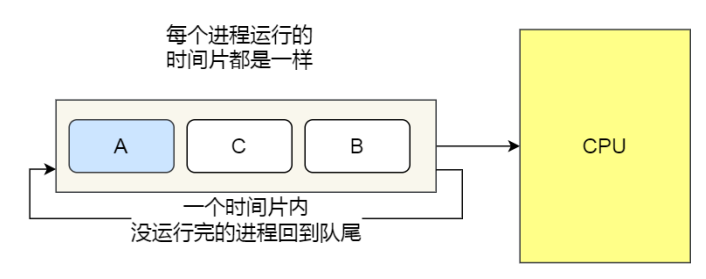
\includegraphics{figures/05-02-04时间片轮转.png}
\end{figure}
(2)npucore进程调度的创新:
npucore团队在进行性能调优的过程中,发现操作系统运行示例程序时,IO操作导致cpu挂起的性能损失很大,因此团队对调度器进行修改,使其支持阻塞式的进程调度模式。

阻塞式和非阻塞式IO是访问设备的两种模式,驱动程序可以灵活的支持两种IO模式。

\textbullet 阻塞操作指的是在执行设备操作时,如果得不到资源,那么进程就会挂起一直到满足可以操作的条件后再进行操作,被挂起的进程会进入睡眠状态,进入阻塞队列中,直到被唤醒。

\textbullet 非阻塞指的是不能进行设备操作时不进行挂起,要么一直等待,要么放弃处理机。

采用阻塞式进程调度模式的好处是显而易见的,不能获取资源的进程将会被休眠,让出CPU供给其他进程,直到得到资源被唤醒,唤醒进程的代码于中断之中,因为在硬件获得资源的同时往往伴随着一个中断。

最后还需要讲的是,npucore中进程的状态,其分为就绪,正在执行,阻塞(interruptible)状态:

\begin{figure}[H]
    \centering
    \caption[short]{进程的状态}
    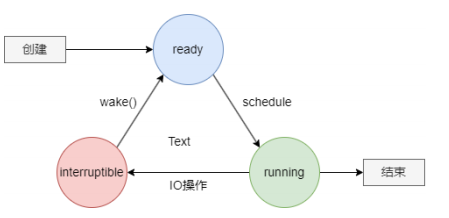
\includegraphics{figures/05-02-04进程状态.png}
\end{figure}


5.2.4.3 进程调度相关代码

前文中我们简要的介绍了何为进程调度以及常见的几种进程调度,还有npucore使用了什么调度策略,接下来我们将根据具体的代码来讲解进程调度。
\\[5pt]

1.进程调度的容器:任务管理器
任务管理器TaskManager是进程调度的容器,其包含一个就绪队列和一个可中断的睡眠状态队列。我们知道,进程由数据结构TCB来描述,而目前正在运行的TCB处于processor(处理器)之中管理,而一台计算机不只有一个进程在工作 ,那些没有在processor上运行的进程TCB则处于任务管理器中的两个队列之中,一部分是可以准备运行的就绪TCB,一部分是处于休眠状态的TCB,该休眠状态可以被中断程序唤醒,因此是可中断的队列。

根据有没有oom_handler特性对于TaskManger有两种数据结构,当有时候,会包含ActiveTracker这个数据结构,这个的作用主要是维护一个位图来跟踪进程的活动状态,可以检查和设置活动状态

\begin{lstlisting}[language=rust,caption={数据结构ActiveTracker}]
    pub struct ActiveTracker {
            bitmap: Vec<u64>,
        }
        
        #[cfg(feature = "oom_handler")]
        #[allow(unused)]
        impl ActiveTracker {
            pub const DEFAULT_SIZE: usize = SYSTEM_TASK_LIMIT;
            pub fn new() -> Self {
                let len = (Self::DEFAULT_SIZE + 63) / 64;
                let mut bitmap = Vec::with_capacity(len);
                bitmap.resize(len, 0);
                Self { bitmap }
            }
            pub fn check_active(&self, pid: usize) -> bool {
                (self.bitmap[pid / 64] & (1 << (pid % 64))) != 0
            }
            pub fn check_inactive(&self, pid: usize) -> bool {
                (self.bitmap[pid / 64] & (1 << (pid % 64))) == 0
            }
            pub fn mark_active(&mut self, pid: usize) {
                self.bitmap[pid / 64] |= 1 << (pid % 64)
            }
            pub fn mark_inactive(&mut self, pid: usize) {
                self.bitmap[pid / 64] &= !(1 << (pid % 64))
            }
        }

\end{lstlisting}

当没有oom_handler特性时TaskManger的数据结构如下:
\begin{lstlisting}[language=rust,caption={数据结构TaskManager}]
    pub struct TaskManager {
    pub ready_queue: VecDeque<Arc<TaskControlBlock>>,
    pub interruptible_queue: VecDeque<Arc<TaskControlBlock>>,
}
\end{lstlisting}
包含了就绪队列和一个可中断的等待队列构成,都是存储进程控制块的队列,其中进程控制块使用原子引用计数智能指针进行引用计数。这有助于有效地管理进程的生命周期和共享。
其中就绪队列ready_queue中存储已准备好运行的进程。

进程在这个队列中等待被调度器选中并执行。当一个进程处于等待 CPU 资源的状态,但是已经准备好执行时,它会被添加到这个队列。

可中断等待队列interruptible_queue专门用于存放处于可中断的睡眠状态的进程,这些进程可以被中断唤醒以继续执行。

关于TaskManger的具体实现如下:
\begin{lstlisting}[language=rust,caption={TaskManager下的方法}]
    impl TaskManager {
    #[cfg(feature = "oom_handler")]
    pub fn new() -> Self {
        Self {
            ready_queue: VecDeque::new(),
            interruptible_queue: VecDeque::new(),
            active_tracker: ActiveTracker::new(),
        }
    }
    #[cfg(not(feature = "oom_handler"))]
    pub fn new() -> Self {
        Self {
            ready_queue: VecDeque::new(),
            interruptible_queue: VecDeque::new(),
        }
    }
    pub fn add(&mut self, task: Arc<TaskControlBlock>) {
        self.ready_queue.push_back(task);
    }
    #[cfg(feature = "oom_handler")]
    pub fn fetch(&mut self) -> Option<Arc<TaskControlBlock>> {
        match self.ready_queue.pop_front() {
            Some(task) => {
                self.active_tracker.mark_active(task.pid.0);
                Some(task)
            }
            None => None,
        }
    }
    #[cfg(not(feature = "oom_handler"))]
    pub fn fetch(&mut self) -> Option<Arc<TaskControlBlock>> {
        self.ready_queue.pop_front()
    }
    pub fn add_interruptible(&mut self, task: Arc<TaskControlBlock>) {
        self.interruptible_queue.push_back(task);
    }
    pub fn drop_interruptible(&mut self, task: &Arc<TaskControlBlock>) {
        self.interruptible_queue
            .retain(|task_in_queue| Arc::as_ptr(task_in_queue) != Arc::as_ptr(task));
    }
    pub fn find_by_pid(&self, pid: usize) -> Option<Arc<TaskControlBlock>> {
        self.ready_queue
            .iter()
            .chain(self.interruptible_queue.iter())
            .find(|task| task.pid.0 == pid)
            .cloned()
    }
    pub fn find_by_tgid(&self, tgid: usize) -> Option<Arc<TaskControlBlock>> {
        self.ready_queue
            .iter()
            .chain(self.interruptible_queue.iter())
            .find(|task| task.tgid == tgid)
            .cloned()
    }
    pub fn ready_count(&self) -> u16 {
        self.ready_queue.len() as u16
    }
    pub fn interruptible_count(&self) -> u16 {
        self.interruptible_queue.len() as u16
    }
    pub fn wake_interruptible(&mut self, task: Arc<TaskControlBlock>) {
        match self.try_wake_interruptible(task) {
            Ok(_) => {}
            Err(_) => {
                log::trace!("[wake_interruptible] already waken");
            }
        }
    }
    pub fn try_wake_interruptible(
        &mut self,
        task: Arc<TaskControlBlock>,
    ) -> Result<(), WaitQueueError> {
        self.drop_interruptible(&task);
        if self.find_by_pid(task.pid.0).is_none() {
            self.add(task);
            Ok(())
        } else {
            Err(WaitQueueError::AlreadyWaken)
        }
    }
    #[allow(unused)]
    // debug use only
    pub fn show_ready(\&self) {
        self.ready_queue.iter().for_each(|task| {
            log::error!("[show_ready] pid: {}", task.pid.0);
        })
    }
    #[allow(unused)]
    // debug use only
    pub fn show_interruptible(\&self) {
        self.interruptible_queue.iter().for_each(|task| {
            log::error!("[show_interruptible] pid: {}", task.pid.0);
        })
    }
}
\end{lstlisting}
\begin{table}[H]
    \centering
    \caption{TaskManager下方法的介绍}
    \begin{tabularx}{17cm}{|X|X|X|X|X|}
        \hline
        方法名 & 目的 & 参数 & 操作 & 返回值 \\
        \hline
        new & 初始化一个TaskManager实例。& 无 & 无 & 返回一个包含两个空队列的TaskManager实例。 \\
        \hline
        add & 将进程添加到就绪队列。 & task: Child(代表一个进程)。 & 无 & 无 \\
        \hline
        fetch & 从就绪队列中获取一个进程。 & 无 & ready_queue头部弹出一个进程,并返回它,如果有oom_handler特性,则将弹出进程标记为活跃状态。 & 返回Option<Child>表示可能获取到的进程。 \\
        \hline
        add_interruptible & 将可中断的进程添加到可中断队列。 & task: Child(代表一个进程)。 & 将 task 添加到 interruptible_queue 尾部。 & 无 \\
        \hline
        drop_interruptible & 从可中断队列中移除指定的可中断进程。 & task:\&Child(代表一个进程)。 & 保留不等于 task 的进程,从而移除了匹配的进程。 & 无 \\
        \hline
        find_by_pid & 根据进程 ID 在队列中查找进程 & pid: usize(进程 ID)。 & 无 & 返回 Option<Child>,表示找到的进程。 \\
        \hline
        find_by_tgid & 根据线程组 ID 在队列中查找进程。 & tgid: usize(线程组 ID)。 & 无 & 返回 Option<Child>,表示找到的进程。 \\
        \hline
        ready_count & 获取就绪队列中进程的数量 & 无 & 无 & 返回 u16 类型的进程数量 \\
        \hline
        interruptible_count	& 获取可中断队列中进程的数量 & 无 & 无 & 返回 u16 类型的进程数量 \\
        \hline
        wake_interruptible & 将已唤醒的可中断进程移动到就绪队列中 & task: Child(代表一个已唤醒的进程) & 调用 try_wake_interruptible 方法,忽略可能的错误 & 无 \\
        \hline
        try_wake_interruptible & 尝试将已唤醒的可中断进程移动到就绪队列中 & task: Child(代表一个已唤醒的进程) & 如果进程不存在于就绪队列中,将其添加到就绪队列中,否则返回错误 & 返回 Result<(), WaitQueueError>,表示操作成功或已经唤醒 \\
        \hline
        show_ready & 仅用于调试,打印就绪队列的进程 PID。这些方法通过入队出队,查找等方法实现了进程的调度。 & 无 & 无 & 无 \\
        \hline
        show_interruptible & 仅用于调试,打印可中断队列的进程 PID。这些方法通过入队出队,查找等方法实现了进程的调度 & 无 & 无 & 无 \\
        \hline
    \end{tabularx}
\end{table}
这是最主要的进程调度的数据结构TaskManger的主要内容,Npucore除了TaskManger提供的两个队列之外还建立了Waitqueue,TimeoutWaitQueue两个队列分别为等待队列和超时等待队列,这两个队列的结构体为:
\begin{lstlisting}[language=rust,caption={数据结构WaitQueue与TimeoutWaitQueue}]
    pub struct WaitQueue {
    inner: VecDeque<Weak<TaskControlBlock>>,
}
pub struct TimeoutWaitQueue {
    inner: BinaryHeap<TimeoutWaiter>,
}
\end{lstlisting}
都接收了TCB的弱引用作为队列元素,在Npucore 中,TaskManger包含的方法实现了最主要的进程调度,WaitQueue和TimeoutWaitQueue则是在进程/线程同步方面Futex的视线中发挥作用

以下是关于WaitQueue的实现:
\begin{lstlisting}[language=rust,caption={数据结构WaitQueue下的方法}]
    impl WaitQueue {
    pub fn new() -> Self {
        Self {
            inner: VecDeque::new(),
        }
    }
    pub fn add_task(&mut self, task: Weak<TaskControlBlock>) {
        self.inner.push_back(task);
    }
    pub fn pop_task(&mut self) -> Option<Weak<TaskControlBlock>> {
        self.inner.pop_front()
    }
    pub fn contains(&self, task: &Weak<TaskControlBlock>) -> bool {
        self.inner
            .iter()
            .any(|task_in_queue| Weak::as_ptr(task_in_queue) == Weak::as_ptr(task))
    }
    pub fn is_empty(&self) -> bool {
        self.inner.is_empty()
    }
    pub fn wake_all(&mut self) -> usize {
        self.wake_at_most(usize::MAX)
    }
    pub fn wake_at_most(&mut self, limit: usize) -> usize {
        if limit == 0 {
            return 0;
        }
        let mut manager = TASK_MANAGER.lock();
        let mut cnt = 0;
        while let Some(task) = self.inner.pop_front() {
            match task.upgrade() {
                Some(task) => {
                    let mut inner = task.acquire_inner_lock();
                    match inner.task_status {
                        super::TaskStatus::Interruptible => {
                            inner.task_status = super::task::TaskStatus::Ready
                        }
                        _ => continue,
                    }
                    drop(inner);
                    if manager.try_wake_interruptible(task).is_ok() {
                        cnt += 1;
                    }
                    if cnt == limit {
                        break;
                    }
                }
            
                None => continue,
            }
        }
        cnt
    }
}
\end{lstlisting}
\begin{table}[H]
    \centering
    \caption{WaitQueue下方法的介绍}
    \begin{tabularx}{17cm}{|X|X|X|X|X|}
        \hline
        方法名 & 目的 & 参数 & 操作 & 返回值 \\
        \hline
        new & 创建一个新的 WaitQueue 实例 & 无 & 初始化内部使用 VecDeque 存储的任务队列 & 新创建的 WaitQueue 实例 \\
        \hline
        add_task & 将一个任务添加到 WaitQueue 中 & 自身引用,task - 用 Weak 包装的任务 & 将任务添加到队列的末尾 & 无 \\
        \hline
        pop_task & 从 WaitQueue 中弹出一个任务 & 无 & 从队列的前端弹出一个任务 & 返回一个 Option,可能是弹出的任务,如果队列为空则为 None \\
        \hline
        contains & 判断 WaitQueue 中是否包含与给定任务相等的元素 & 自身引用,task-要判断的任务 & 比较任务的指针是否相等 & 如果队列中包含相等的任务则返回 true,否则返回 false \\
        \hline
        is_empty & 判断 WaitQueue 是否为空 & 自身引用 & 检查内部队列是否为空 & 如果队列为空则返回 true,否则返回 false \\
        \hline
        wake_all & 唤醒 WaitQueue 中的所有任务 & 自身可变引用 & 将所有任务的状态更改为 Ready & 返回实际唤醒的任务数量 \\
        \hline
        wake_at_most & 唤醒 WaitQueue 中不超过 limit 数量的任务 & 自身可变引用,limit - 最大唤醒数量 & 将不超过 limit 数量的任务状态更改为 Ready & 返回实际唤醒的任务数量 \\
        \hline
    \end{tabularx}
\end{table}

以下是关于TimeoutWaitQueue的实现:

\begin{lstlisting}[language=rust,caption={TimeoutWaitQueue下的方法}]
    impl TimeoutWaitQueue {
    pub fn new() -> Self {
        Self {
            inner: BinaryHeap::new(),
        }
    }
    pub fn add_task(&mut self, task: Weak<TaskControlBlock>, timeout: TimeSpec) {
        self.inner.push(TimeoutWaiter { task, timeout });
    }
    pub fn wake_expired(&mut self, now: TimeSpec) {
        let mut manager = TASK_MANAGER.lock();
        while let Some(waiter) = self.inner.pop() {
            // the remaining tasks in heap haven't reach their timeout
            if waiter.timeout > now {
                log::trace!(
                    "[wake_expired] no more expired, next pending task timeout: {:?}, now: {:?}",
                    waiter.timeout,
                    now
                );
                self.inner.push(waiter);
                break;
            // wake one task
            } else {
                match waiter.task.upgrade() {
                    Some(task) => {
                        let mut inner = task.acquire_inner_lock();
                        match inner.task_status {
                            super::TaskStatus::Interruptible => {
                                inner.task_status = super::task::TaskStatus::Ready
                            }
                            _ => continue,
                        }
                        drop(inner);
                        log::trace!(
                            "[wake_expired] pid: {}, timeout: {:?}",
                            task.pid.0,
                            waiter.timeout
                        );
                        manager.wake_interruptible(task);
                    }
                    None => continue,
                }
            }
        }
    }
    #[allow(unused)]
    // debug use only
    pub fn show_waiter(&self) {
        for waiter in self.inner.iter() {
            log::error!("[show_waiter] timeout: {:?}", waiter.timeout);
        }
    }
}
\end{lstlisting}
\begin{table}[H]
    \caption{TimeoutWaitQueue下的方法的介绍}
    \begin{tabularx}{17cm}{|X|X|X|X|X|}
        \hline
        方法名 & 目的 & 参数 & 操作 & 返回值 \\
        \hline
        new & 创建一个新的 TimeoutWaitQueue 实例 & 无 & 初始化内部使用 BinaryHeap 存储的超时等待队列 & 新创建的 TimeoutWaitQueue 实例 \\
        \hline
        add_task & 将一个带有超时时间的任务添加到 TimeoutWaitQueue 中 & 自身可变引用,task - 用 Weak 包装的任务。timeout - 任务的超时时间。 &  将任务包装成 TimeoutWaiter 结构,并将其按照超时时间顺序插入二进制堆中 & 无 \\
        \hline
        wake_expired & 唤醒 TimeoutWaitQueue 中已经超时的任务 & 自身可变引用,now-当前时间 & 弹出二进制堆顶部的任务,检查其超时时间是否已经到达。如果任务还未超时,将其重新插入堆中并结束。如果任务已经超时,将任务的状态更改为 Ready,并唤醒对应的任务。 & 无 \\
        \hline
        show_waiter & 用于调试,打印当前 TimeoutWaitQueue 中的等待者(任务)的超时时间 & 自身引用 & 打印每个等待者的超时时间 & 无 \\
        \hline
    \end{tabularx}
\end{table}

2.阻塞式进程调度的实现:

多路复用:

多路复用的实现如下:当一个进程等待磁盘请求时,OS 使之进入睡眠状态,然后调度执行另一个进程。另外,当一个进程耗尽了它在处理器上运行的时间片后,OS 使用时钟中断强制它停止运行,这样调度器才能调度运行其他进程。这样的多路复用机制为进程提供了独占处理器的假象,类似于OS 使用内存分配器和页表硬件为进程提供了独占内存的假象。

实现多路复用有几个难点。首先,应该如何从运行中的一个进程切换到另一个进程?OS 采用了普通的上下文切换机制;虽然这里的思想是非常简洁明了的,但是其代码实现是操作系统中最晦涩难懂的一部分。第二,如何让上下文切换透明化?OS 只是简单地使用时钟中断处理程序来驱动上下文切换。第三,可能出现多个 CPU 同时切换进程的情况,那么我们必须使用一个带锁的方案来避免竞争。第四,进程退出时必须释放其占用内存与资源,但由于它本身在使用自己的资源(譬如其内核栈),所以不能由该进程本身释放其占有的所有资源。

OS 必须为进程提供互相协作的方法。譬如,父进程需要等待子进程结束,以及读取管道数据的进程需要等待其他进程向管道中写入数据。与其让这些等待中的进程消耗 CPU 资源,不如让它们暂时放弃 CPU,进入睡眠状态来等待其他进程发出事件来唤醒它们。但我们必须要小心设计以防睡眠进程遗漏事件通知。

上下文切换:

如下图所示,OS 在低层次中实现了两种上下文切换:从进程的内核线程切换到当前 CPU 的调度器线程,从调度器线程到进程的内核线程。OS 永远不会直接从用户态进程切换到另一个用户态进程;这种切换是通过用户态-内核态切换(系统调用或中断)、切换到调度器、切换到新进程的内核线程、最后这个陷入返回实现的。我们将以一个简单的例子,详细介绍了这一过程。

\begin{figure}[H]
    \centering
    \caption[short]{上下文切换}
    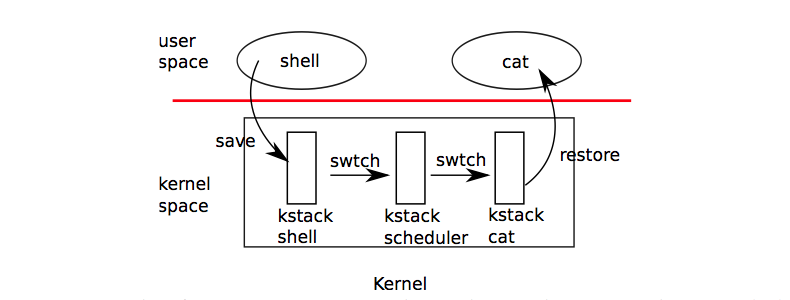
\includegraphics{figures/05-02-04上下文切换.png}
\end{figure}

设有两个用户态进程 A 和 B,它们在操作系统内核的管理下运行。CPU 当前正在执行进程 A。

首先是用户态到内核态的切换。当进程 A 需要执行一个系统调用(例如,读写文件、申请内存等)或者发生一个中断事件(例如,时钟中断、硬件中断等),CPU 会触发一个异常或中断,将控制权转移到操作系统内核。

触发异常或中断: 比如,进程 A执行了一个系统调用指令或硬件设备触发了中断。

保存用户态上下文: 操作系统内核保存进程 A 的用户态上下文,包括通用寄存器、程序计数器、堆栈指针等。

切换到内核态: CPU 转到内核态执行,此时操作系统内核可以访问更多的特权指令和数据结构。

其次是在内核态的处理过程。在内核态,操作系统会执行一些必要的操作,比如:

\quad  \textbullet 系统调用处理: 根据系统调用的类型,执行相应的内核代码完成用户请求的操作。

\quad  \textbullet 调度器的工作: 决定下一个要执行的进程。这可能涉及到选择一个就绪队列中的新进程。

内核线程切换: 如果需要切换到一个新的用户态进程(假设是进程 B),操作系统可能会将控制权切换到该进程的内核线程。

之后为内核态到用户态的切换:

\quad \textbullet 恢复用户态上下文: 如果切换到了新的用户态进程 B,操作系统会从进程 B 的内核线程中恢复用户态上下文。

\quad \textbullet 切换到用户态: CPU 会从内核态切换回用户态,开始执行进程 B 的用户态代码。

最后,进程 B 开始执行:

\quad \textbullet 加载用户态上下文: 进程 B 的用户态上下文被加载到 CPU 寄存器中。
	
\quad \textbullet 继续执行: CPU 开始执行进程 B 的用户态代码,从上次中断或系统调用的位置继续执行。

整个过程中,关键的步骤包括从用户态到内核态的切换,内核态的处理过程,以及从内核态回到用户态的切换。这个过程确保了不同进程之间的无缝切换,使得操作系统能够有效地进行多任务调度。

任务切换:

当一台计算机开始运行时,操作系统首先会通过懒分配创建一个初始的进程,该进程是一个全局的进程,接下来的进程都由它创建。初始进程创建以后,根据计算机的需要或者用户的操作,操作系统开始由clone函数来创建一个个新的进程并加入到就绪队列中。按照时间片
轮转的想法,操作系统给正在处理器上运行的(也就是processor所拥有的TCB)进程分配了一个时间片,在自然运行到时间耗尽后,操作系统就会使用sys_yield()函数让出当前进程对处理器的占有权,又或者内核出现错误造成trap,程序也会使当前进程让出处理器,其中的核心函数便是suspend_current_and_run_next,该函数将当前进程的上下文进行保存,并将进程的状态改成ready,表示进程准备执行,然后将他放回到ready队列中的队尾进行排队,等待下一次轮转到它。

suspend_current_and_run_next函数会使得当前进程从current_task切换到中转进程idle,而调度器如何将idle切换为next_task呢?

它将使用run_tasks()函数完成从idle到next_task的切换。run_tasks()函数位于os/src/task/processor.rs下。让我们看 os/src/task/processor.rs 下的 run_task 函数:
\begin{lstlisting}[language=rust,caption={run_task函数}]
    pub fn run_tasks() {
    loop {
        let mut processor = PROCESSOR.lock();
        if let Some(task) = fetch_task() {
            let idle_task_cx_ptr = processor.get_idle_task_cx_ptr();
            // access coming task TCB exclusively
            let next_task_cx_ptr = {
                let mut task_inner = task.acquire_inner_lock();
                task_inner.task_status = TaskStatus::Running;
                &task_inner.task_cx as *const TaskContext
            };
            processor.current = Some(task);
            // release processor manually
            drop(processor);
            unsafe {
                __switch(idle_task_cx_ptr, next_task_cx_ptr);
            }
        } else {
            drop(processor);
            // we have no ready tasks, try to wake some...
            do_wake_expired();
        }
    }
}
\end{lstlisting}

可以看到,操作系统采⽤"轮询机制",在操作系统运⾏的任⼀时刻都在尝试从idle流切换到下一个进程(采用loop死循环),接着我们分析⼀下具体的过程。

fetch_task() 的作用是选取⼀个将要执⾏的进程 

\begin{lstlisting}[language=rust,caption={fetch_task函数}]
    pub fn fetch_task() -> Option<Arc<TaskControlBlock>> { 
TASK_MANAGER.lock().fetch() 
}
impl TaskManager { 
//... 
pub fn fetch(&mut self) -> Option<Arc<TaskControlBlock>> { 
self.ready_queue.pop_front() 
} 
//... 
} 
\end{lstlisting}

可以看到,调度器的选择是将“就绪任务”的队列进⾏出队操作。
因此我们可以知道, NPUcore 中对进程的调度实际上就是对 ready_queue 进行管理。 

等待队列:

进程的调度过程中,有一些进程是需要等待某种资源,例如IO输入这样的资源,因此才陷入阻塞过程中,他们不得到自己所需的资源前,便无法被唤醒加入就绪队列中(因此它不同于interruptible_queue中的进程,在可中断睡眠队列中的进程,需要等待中断操作就可以被唤醒),因此这涉及到了waitqueue这个重要的数据结构。

等待队列(wait_queue)是用于管理等待特定资源或时间的进程或线程,它是一种先进先出的数据结构。该队列通常用于解决并发编程中的同步和互斥问题。当多个进程或者线程需要访问共享资源时,如果资源已经被占用,那么需要将正在等待的进程放入等待队列,以便在资源可用时依次获得访问权限。

当某资源得到释放,是的等待队列中的进程可被唤醒时,操作系统会调用wake_at_most这个方法。

\begin{lstlisting}[language=rust,caption={wake_at_most方法}]
    pub fn wake_at_most(&mut self, limit: usize) -> usize {
        if limit == 0 {
            return 0;
        }
        let mut manager = TASK_MANAGER.lock();
        let mut cnt = 0;
        while let Some(task) = self.inner.pop_front() {
            match task.upgrade() {
                Some(task) => {
                    let mut inner = task.acquire_inner_lock();
                    match inner.task_status {
                        super::TaskStatus::Interruptible => {
                            inner.task_status = super::task::TaskStatus::Ready
                        }
                        _ => continue,
                    }
                    drop(inner);
                    if manager.try_wake_interruptible(task).is_ok() {
                        cnt += 1;
                    }
                    if cnt == limit {
                        break;
                    }
                }
                None => continue,
            }
        }
        cnt
    }
\end{lstlisting}
该函数的功能为:从等待队列中唤醒最多limit个任务,并返回实际唤醒的任务数量。\\
首先,函数检查limit是否为0,如果为0,则表示没有唤醒任何任务。\\
然后,函数获取全局的任务管理器的锁,确保任务管理器的线程安全性。\\
接下来,函数使用cnt记录唤醒的任务的数量,初始为0.\\
然后,函数进入循环,从等待队列(self.inner)的头部弹出任务,并进行处理。\\
在处理吃钱,函数会尝试将任务引用升级为ARC类型的对象。如果该对象有效,则执行以下操作:\\
1)获取任务对象的内部锁(acquire_inner_lock)\\
2)根据任务的状态进行不同处理,interruptible的任务,将其状态设置为ready,如果为其他状态,则不需要唤醒,继续处理下一个任务。\\
3)释放任务对象的内部锁(drop(inner))\\
4)尝试使用try_wake_interruptible方法唤醒任务\\
5)检查cnt计数器是否达到limit限制,达到则跳出循环。\\
如果任务对象引用升级为None,表示任务已经被销毁了,函数会处理下一个任务。\\
最后返回唤醒的任务数量cnt。\\

经过该函数的处理,那些得到了资源的进程,可以被唤醒进入ready队列中,等待时间片的轮转。而该函数中又涉及到了一个关键的函数try_wake_interruptible:

\begin{lstlisting}[language=rust,caption={try_wake_interruptible方法}]
    pub fn try_wake_interruptible(
        &mut self,
        task: Arc<TaskControlBlock>,
    ) -> Result<(), WaitQueueError> {
        self.drop_interruptible(&task);
        if self.find_by_pid(task.pid.0).is_none() {
            self.add(task);
            Ok(())
        } else {
            Err(WaitQueueError::AlreadyWaken)
        }
    }
\end{lstlisting}
该函数接受一个任务对象task作为参数,并尝试唤醒该任务,返回一个result类型,表示唤醒操作的结果。\\
首先,函数调用self.drop_interruptible方法,该方法会从等待队列中移除具有相同pid的任务。该步骤确保在唤醒任务之前先将其从等待队列中移除,避免重复唤醒。\\
接下来,函数使用self.find_by_pid方法来检查ready队列中是否具有相同pid的任务,如果返回None,表示不存在。\\
在这种情况下,函数调用self.add方法将任务添加到准备队列中,并返回ok结果。\\
如果ready队列中具有相同pid的任务,那么函数表示唤醒失败,已经唤醒。\\

除了等待队列以外,还有一个也很重要的数据结构被用在进程的调度中,那就是TimeoutWaitQueue(超时等待池)。

超时等待池用于处理等待超时的情况。在某些场景下,等待某个资源或者事件的进程或线程可能需要在一定的时间内得到相应,如果超过指定时间仍然没有得到响应,那么就需要采取相应的措施。超时等待池允许进程或者线程设置一个超时时间,如果超过时间却未能唤醒,那么就会触发超时逻辑。

超时等待池的存在是为了处理等待时间的限制,以避免进程或者线程在等待资源或时间上长时间阻塞。它提供了一种在等待超时后继续执行的机制,从而增加了系统的可靠性和响应性。

npucore依靠定时器在一定的时间间隔下进入trap,自动唤醒超时等待池中的进程。

在os/src/trap/mod.rs源文件中的trap_handle函数中有对SupervisorTimer中断的处理方式:

\begin{lstlisting}[language=rust,caption={trap_handler中对SupervisorTimer中断的处理}]
            Trap::Interrupt(Interrupt::SupervisorTimer) => {
            do_wake_expired();
            set_next_trigger();
            suspend_current_and_run_next();
        }
\end{lstlisting}
该函数首先调用了do_wake_expired方法:
\begin{lstlisting}[language=rust,caption={do_wake_expired方法}]
    pub fn do_wake_expired() {
    TIMEOUT_WAITQUEUE
        .lock()
        .wake_expired(crate::timer::TimeSpec::now());
}
\end{lstlisting}
其中又调用了TimeoutWaitQueue的wake_expired方法:
\begin{lstlisting}[language=rust,caption={wake_expired方法}]
        pub fn wake_expired(&mut self, now: TimeSpec) {
        let mut manager = TASK_MANAGER.lock();
        while let Some(waiter) = self.inner.pop() {
            // the remaining tasks in heap haven't reach their timeout
            if waiter.timeout > now {
                log::trace!(
                    "[wake_expired] no more expired, next pending task timeout: {:?}, now: {:?}",
                    waiter.timeout,
                    now
                );
                self.inner.push(waiter);
                break;
            // wake one task
            } else {
                match waiter.task.upgrade() {
                    Some(task) => {
                        let mut inner = task.acquire_inner_lock();
                        match inner.task_status {
                            super::TaskStatus::Interruptible => {
                                inner.task_status = super::task::TaskStatus::Ready
                            }
                            _ => continue,
                        }
                        drop(inner);
                        log::trace!(
                            "[wake_expired] pid: {}, timeout: {:?}",
                            task.pid.0,
                            waiter.timeout
                        );
                        manager.wake_interruptible(task);
                    }
                    None => continue,
                }
            }
        }
    }
\end{lstlisting}
该方法获取一个队self的可变引用,以及一个类型为timespec的now参数,没有指定返回来类型。该方法的作用是从任务列表中唤醒已经过期的任务,并将其状态改为ready。
\\[10pt]
首先代码通过获取task_manager对象上的锁来创建一个manager变量,并获取一个互斥锁的保护。\\
接着,代码进入循环,不断的从self.inner弹出一个元素来遍历任务。\\
在循环的每一次迭代中,检查当前任务(waiter)是否已经过期,如果没有过期,代码会将任务放回self.inner,并中断循环。\\
如果任务已经过期,代码会尝试将任务唤醒。它通过调用waiter.task.upgrade()获取任务的强引用。如果任务仍然存在,那么获取内部锁,检查任务状态。\\
如果状态为interruptible,则改为 ready,表示就绪。\\
最后,代码释放内部锁,调用wake_interruptible(task)来唤醒任务。\\
如果任务的强引用已经无效,则说明任务已经被销毁,代码忽略此任务,继续处理下一个任务。
\\[10pt]

由此,我们就讲完了npucore中进程调度相关的内容,本节我们只对重要的地方做了比较详细的介绍,实际上进程的调度是个复杂的问题,光靠这些短短的文字是讲不清楚的,读者可以在闲暇之余,查询网上资料加深自己对进程调度的了解




